\documentclass[10pt,titlepage]{jsarticle}
\usepackage{listings}
\usepackage{jlisting}
\usepackage[T1]{fontenc}
\usepackage{textcomp}
\usepackage{ascmac}
\usepackage[dvipdfmx]{graphicx}
\usepackage{array}
\usepackage{float}
\usepackage{moreverb}
\usepackage{framed}

\renewcommand{\lstlistingname}{ソースコード}
\lstset{
  language=c,
  basicstyle=\ttfamily\scriptsize,
  commentstyle=\textit,
  classoffset=1,
  keywordstyle=\bfseries,
  frame=tRBl,
  framesep=5pt,
  showstringspaces=false,
  numbers=left,
  stepnumber=1,
  numberstyle=\tiny,
  tabsize=2,
  breaklines=true
}
\setcounter{page}{1}

\title{シミュレーション}
\author{4年電子情報工学科\\34番 横前洸佑}
\date{提出日:2019/12/12(木)\\	提出期限:2019/12/12(木)17:00}
\begin{document}

\maketitle

\section{課題1}
\label{sec:kadai1}
課題\ref{sec:kadai1}では、台形公式、式(\ref{eq:daikei})を用いて式(\ref{eq:kadai1})について数値積分を行う。さらに、台形公式を使用する際に分割数を1,2,4,...のように1/2ずつ細かくしていき、台形公式で求めた積分値の結果と解析解との関係を報告する。


\begin{equation}
\label{eq:daikei}
	\int_a^b f(x) dx \approx \frac{h}{2}\left[y_0+2 \sum_{j=1}^{n-1}y_j+y_n\right]
\end{equation}


\begin{equation}
\label{eq:kadai1}
	\int_0^\frac{\pi}{6} \frac{dx}{\cos x}
\end{equation}

\subsection{作成したプログラム}
今回作成したプログラムをソースコード\ref{src:prog1}に示す。

\lstinputlisting[caption=課題1のプログラム,label=src:prog1]{src/kadai1.c}

%%%%%%%%%%%%%%プログラムの説明
このプログラムでは、分割数Nを1から512まで計算している。
そして、計算結果と式\ref{eq:kadai1}の解析解の$\frac{1}{2}\log_e3=0.549306144$との差を表示する。なお、積分される関数及び台形公式の計算部分は使いやすくするためにそれぞれ個別の関数にしている。

\subsection{プログラムの実行結果}
実行結果を以下に示す。
\begin{oframed}
\verbatimtabinput[2]{result/kadai1.txt}
\end{oframed}



\subsection{考察}

計算結果と解析解との差の様子を図\ref{fig:kadai1}に示す。
\begin{figure}[H]
\centering
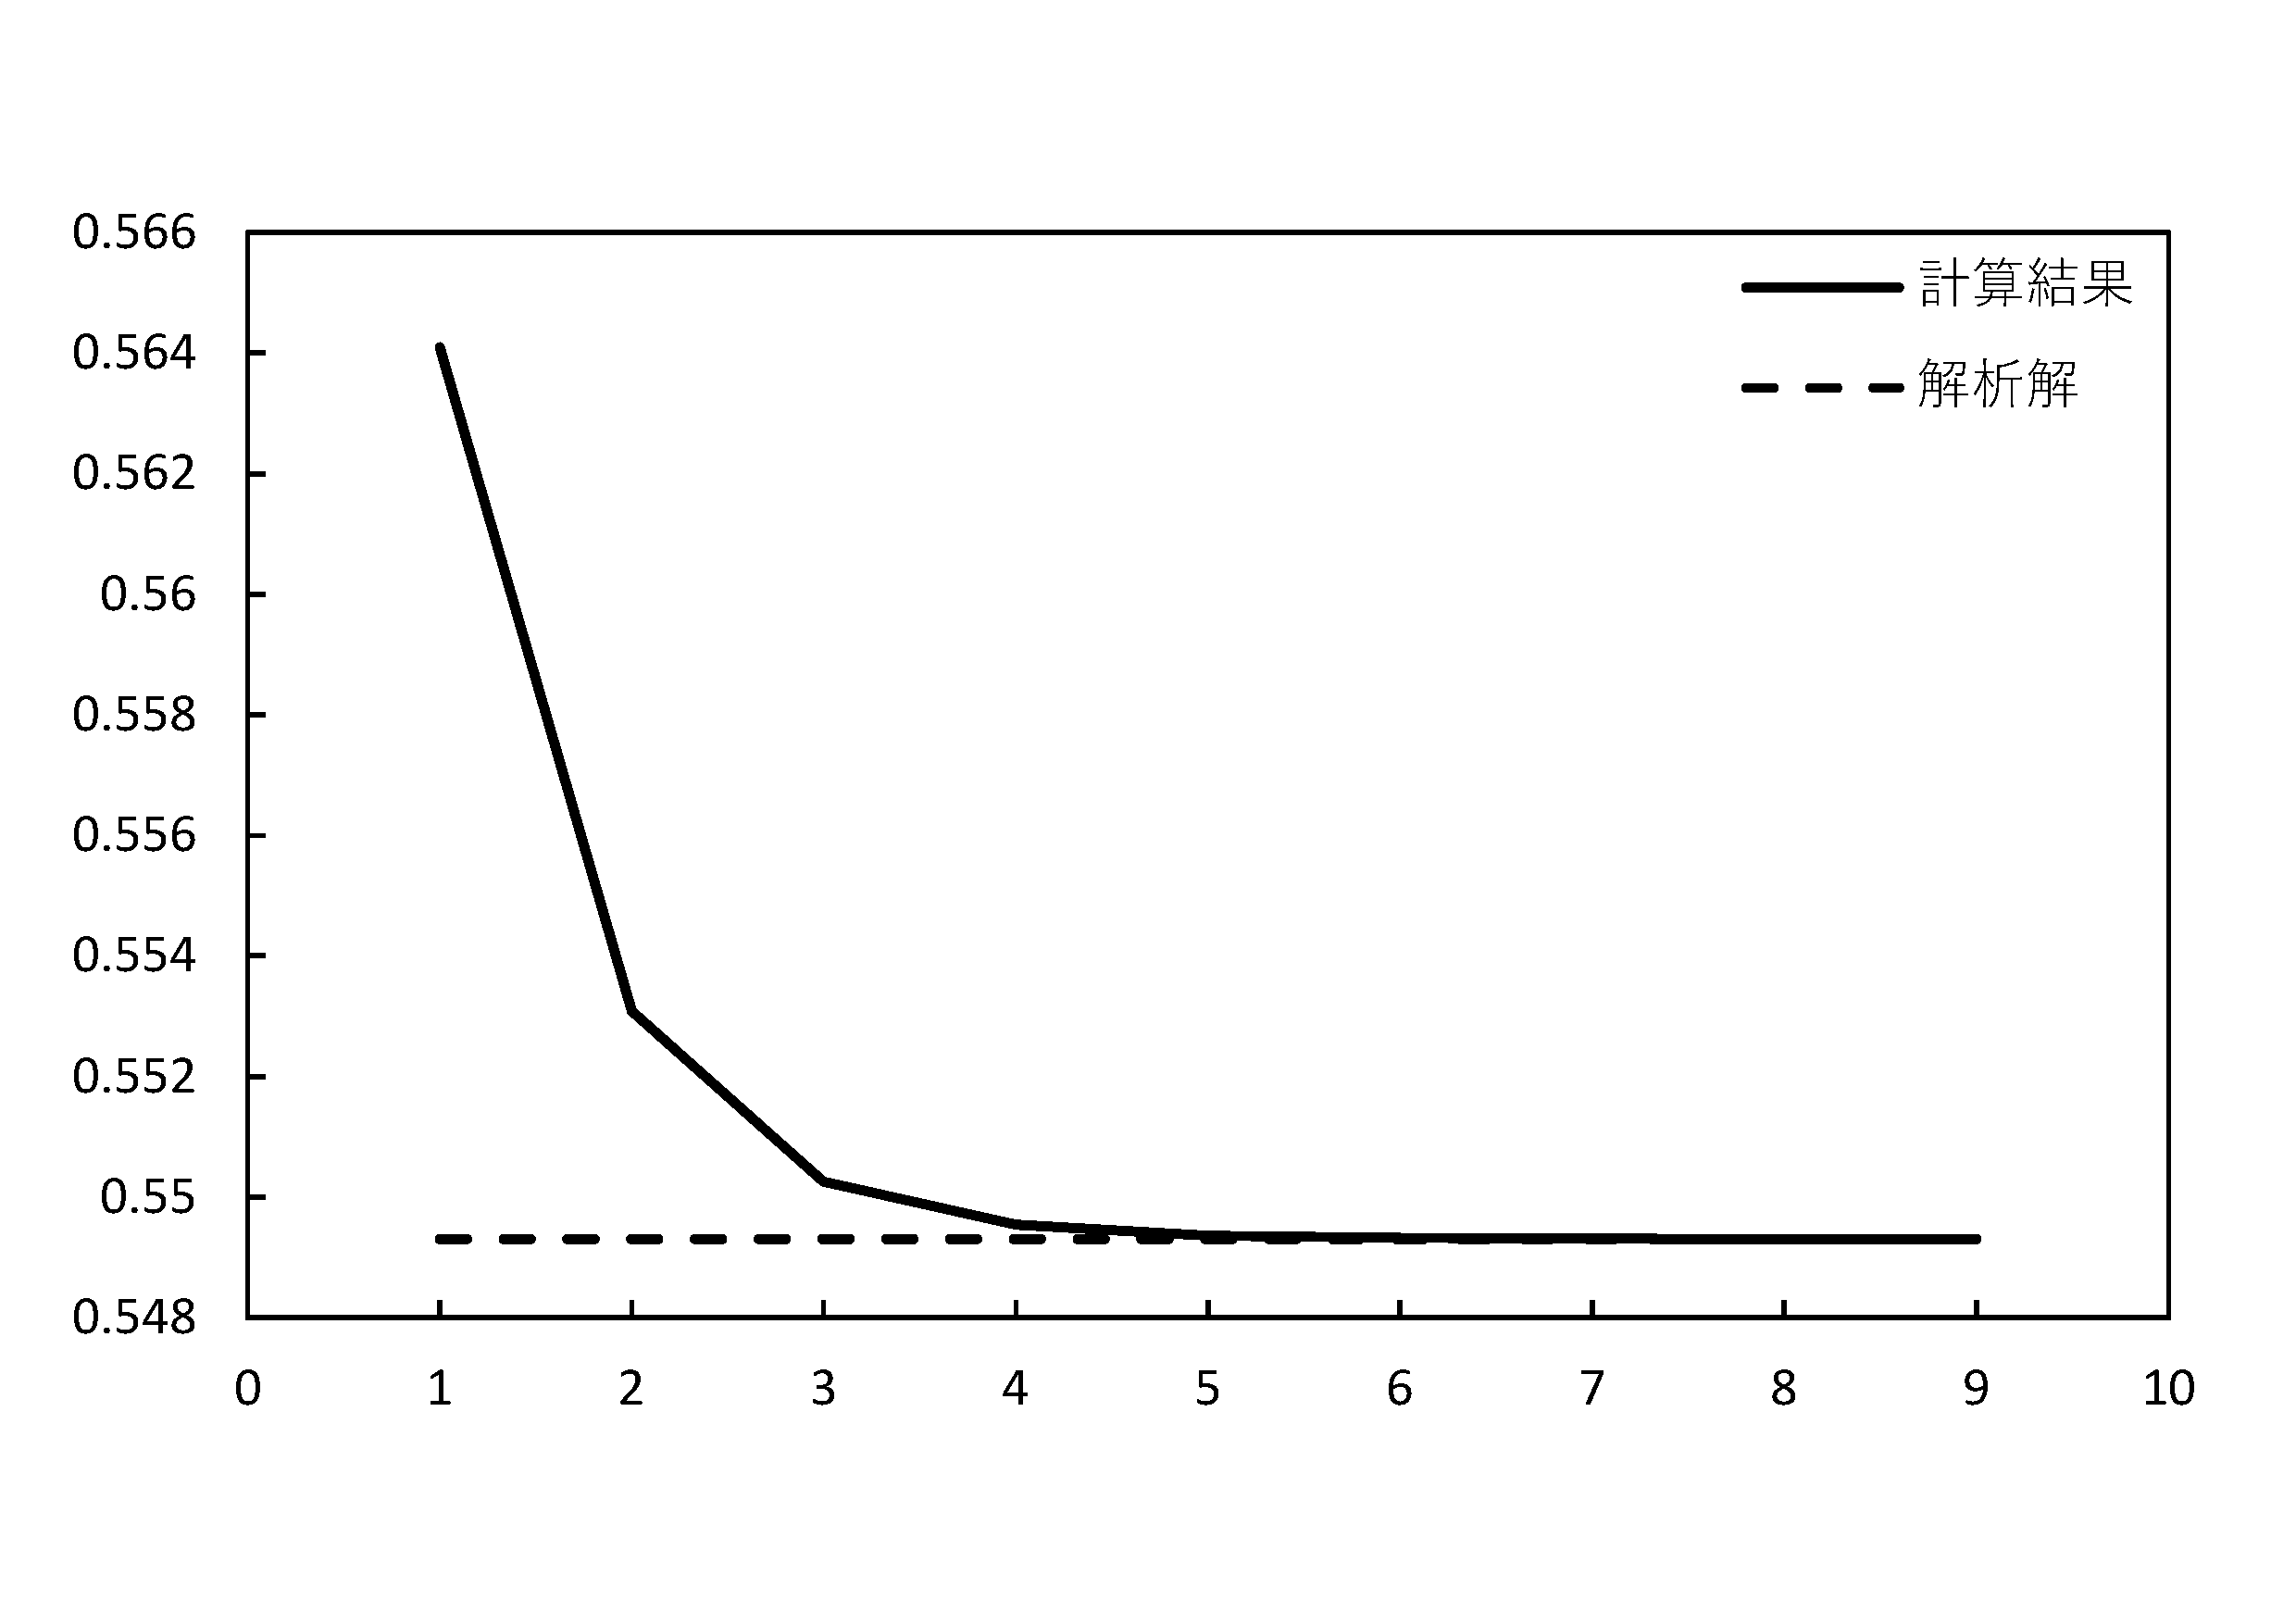
\includegraphics[width=12cm]{img/kadai1.png}
\caption{計算結果と解析解の差の様子}
\label{fig:kadai1}
\end{figure}
実行結果より、分割数Nが1/2になるごとに計算誤差が1/4ずつ減っていることがわかる。
また、図\ref{fig:kadai1}より、分割数Nが増えるたびに計算結果と解析解の差が減って誤差が減って行くことが確認できる。

\section{課題2}
\label{sec:kadai2}

課題\ref{sec:kadai2}では、シンプソンの公式、式(\ref{eq:simpson})を用いて式(\ref{eq:kadai2})について数値積分を行う。さらに{\tt float}型と{\tt double}型で実行し、丸め誤差が現れる刻み幅を調べる。また、刻み幅を1/2にした時の誤差の減り方について報告する。

\begin{equation}
\label{eq:simpson}
	\int_a^b f(x) dx \approx \frac{h}{3}[y_0+4(y_1+y_3+\cdots+y_{n-1})+2(y_2+y_4+\cdots+y_{n-2})+y_n]
\end{equation}

\begin{equation}
\label{eq:kadai2}
	\int_0^\frac{\pi}{2} \sin x dx
\end{equation}

\subsection{作成したプログラム}
今回作成したプログラムをソースコード\ref{src:prog2}に示す。

\lstinputlisting[caption=課題2のプログラム,label=src:prog2]{src/kadai2.c}

%%%%%%%%%%%%%%%%%%%%%%%%プログラムの説明
このプログラムでは、{\tt float}型と{\tt double}型でシンプソンの公式を実行する。そして、(計算結果ー真値)の絶対値を表示している。なお、式(\ref{eq:kadai2})の真値は$1.0$である。また、刻み幅Nは2から50まで計算している。

\subsection{プログラムの実行結果}
実行結果を以下に示す。
\begin{oframed}
\verbatimtabinput[2]{result/kadai2.txt}
\end{oframed}

%%%%%%%%%%%結果解説

\subsection{考察}
実行結果より、丸め誤差が現れる刻み幅は16であることがわかる。
また、刻み幅を1/2にしていった時の誤差の減り方の様子を図\ref{fig:kadai2}に示す。

図\ref{fig:kadai2}は片対数グラフであるため、誤差は指数関数的に減って行くことが確認できる。
\begin{figure}[H]
\centering
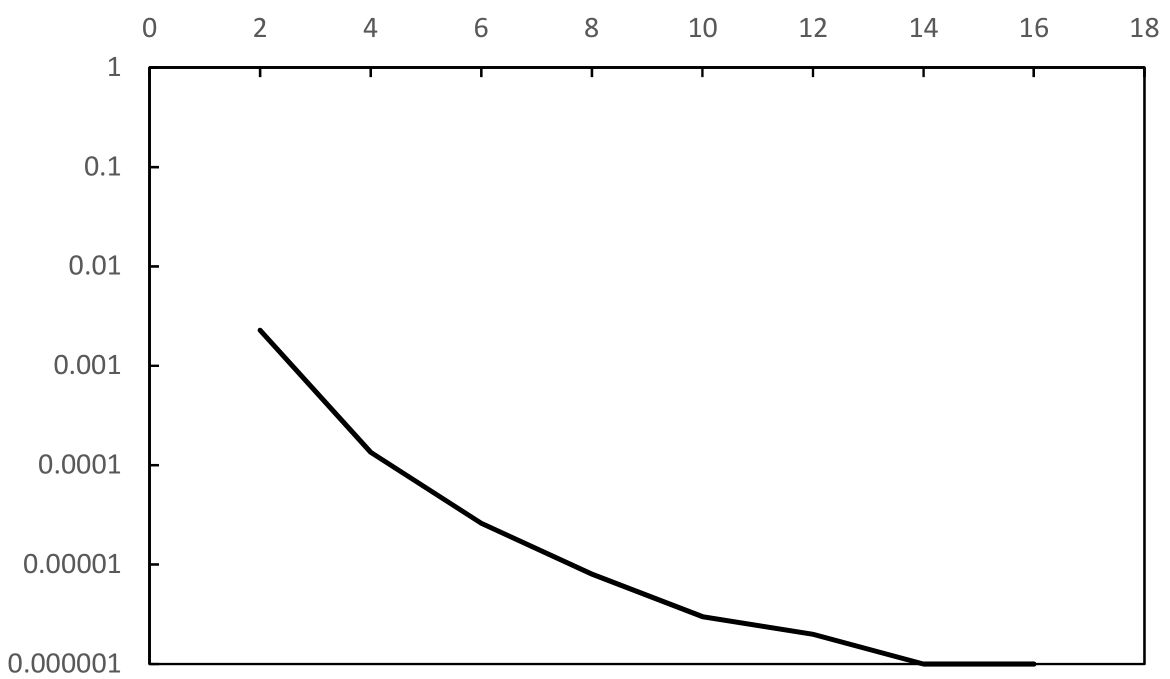
\includegraphics[width=12cm]{img/kadai2.png}
\caption{誤差の減少の様子}
\label{fig:kadai2}
\end{figure}


\section{課題3,4,5}
課題3では、オイラー法を用いて式(\ref{eq:kadai345})の微分方程式を解く。そして、解析解と数値解を同じグラフにプロットし、オイラー法がどの程度正しいかを報告する。

課題4では、課題3をホイン法を用いて同様に行う。また、誤差の特徴についても同様に調べる。

課題5では、課題3をルンゲクッタ法を用いて同様に行う。また、誤差の特徴についても同様に調べる。

\begin{equation}
\label{eq:kadai345}
	\frac{du}{dt} = u (ただし、t=0のときu=1)
\end{equation}	

\begin{itembox}[l]{オイラー法}
\centering
	$x_{i+1}=x_i+h$ \\
	$y_{i+1}=y_i+hf(x_i,y_i)$ 
\end{itembox}

\begin{itembox}[l]{ホイン法}
\centering
	$x_{i+1}=x_i+h$\\
	$k_1=hf(x_i,y_i)$\\
	$k_2=hf(x_i+h,y_i+k_1)$\\
	$y_{i+1}=y_i+\frac{1}{2}(k_1+k_2)$
\end{itembox}

\begin{itembox}[l]{ルンゲ・クッタ法}
\centering
	$x_{i+1}=x_i+h$\\
	$k_1=hf(x_i,y_i)$\\
	$k_2=hf\left(x_i+\frac{h}{2},y_i+\frac{k_1}{2}\right)$\\
	$k_3=hf \left(x_i+\frac{h}{2},y_i+\frac{k_2}{2}\right)$\\
	$k_4=hf\left(x_i+h,y_i+k_3\right)$\\
	$y_{i+1}=y_i+\frac{1}{6}\left(k_1+2k_2+2k_3+k_4\right)$\\
\end{itembox}

式(\ref{eq:kadai345})の解析解は、

\[\frac{du}{dt} = u\]
\[\int \frac{1}{u}du=\int dt\]
\[\log |u|=t+c\]
\[u(t)=\pm e^{t+c}=\pm e^c e^t\]
ここで、$C=\pm e^c$とすると
\[u(t)=Ce^t\]
初期条件より、
\[u_0=Ce^0\]
\[C=1\]
よって
\[u(t)=e^t\]

\subsection{作成したプログラム}
今回作成したプログラムをソースコード\ref{src:prog345}に示す。

\lstinputlisting[caption=課題3、4、5のプログラム,label=src:prog345]{src/kadai345.c}

%%%%%%%%%%プログラムの説明

\subsection{プログラムの実行結果}
実行結果を以下に示す。なお、出力される数値データが多いため、実行結果を一部省略し、$t$の値が$0.10$と$1.00$の時のみを示している。出力された全データは\ref{kadai345}に示す。
\begin{oframed}
\verbatimtabinput[2]{result/kadai345.txt}
\end{oframed}

%%%%%%%%%%%結果解説

\subsection{考察}
図\ref{fig:kadai3}はオイラー法で式(\ref{eq:kadai345})を解いて、刻み幅を$h=0.1,h=0.05,h=0.025$に変更していき同じ$t$の値をグラフにプロットしたものである。

\begin{figure}[H]
\centering
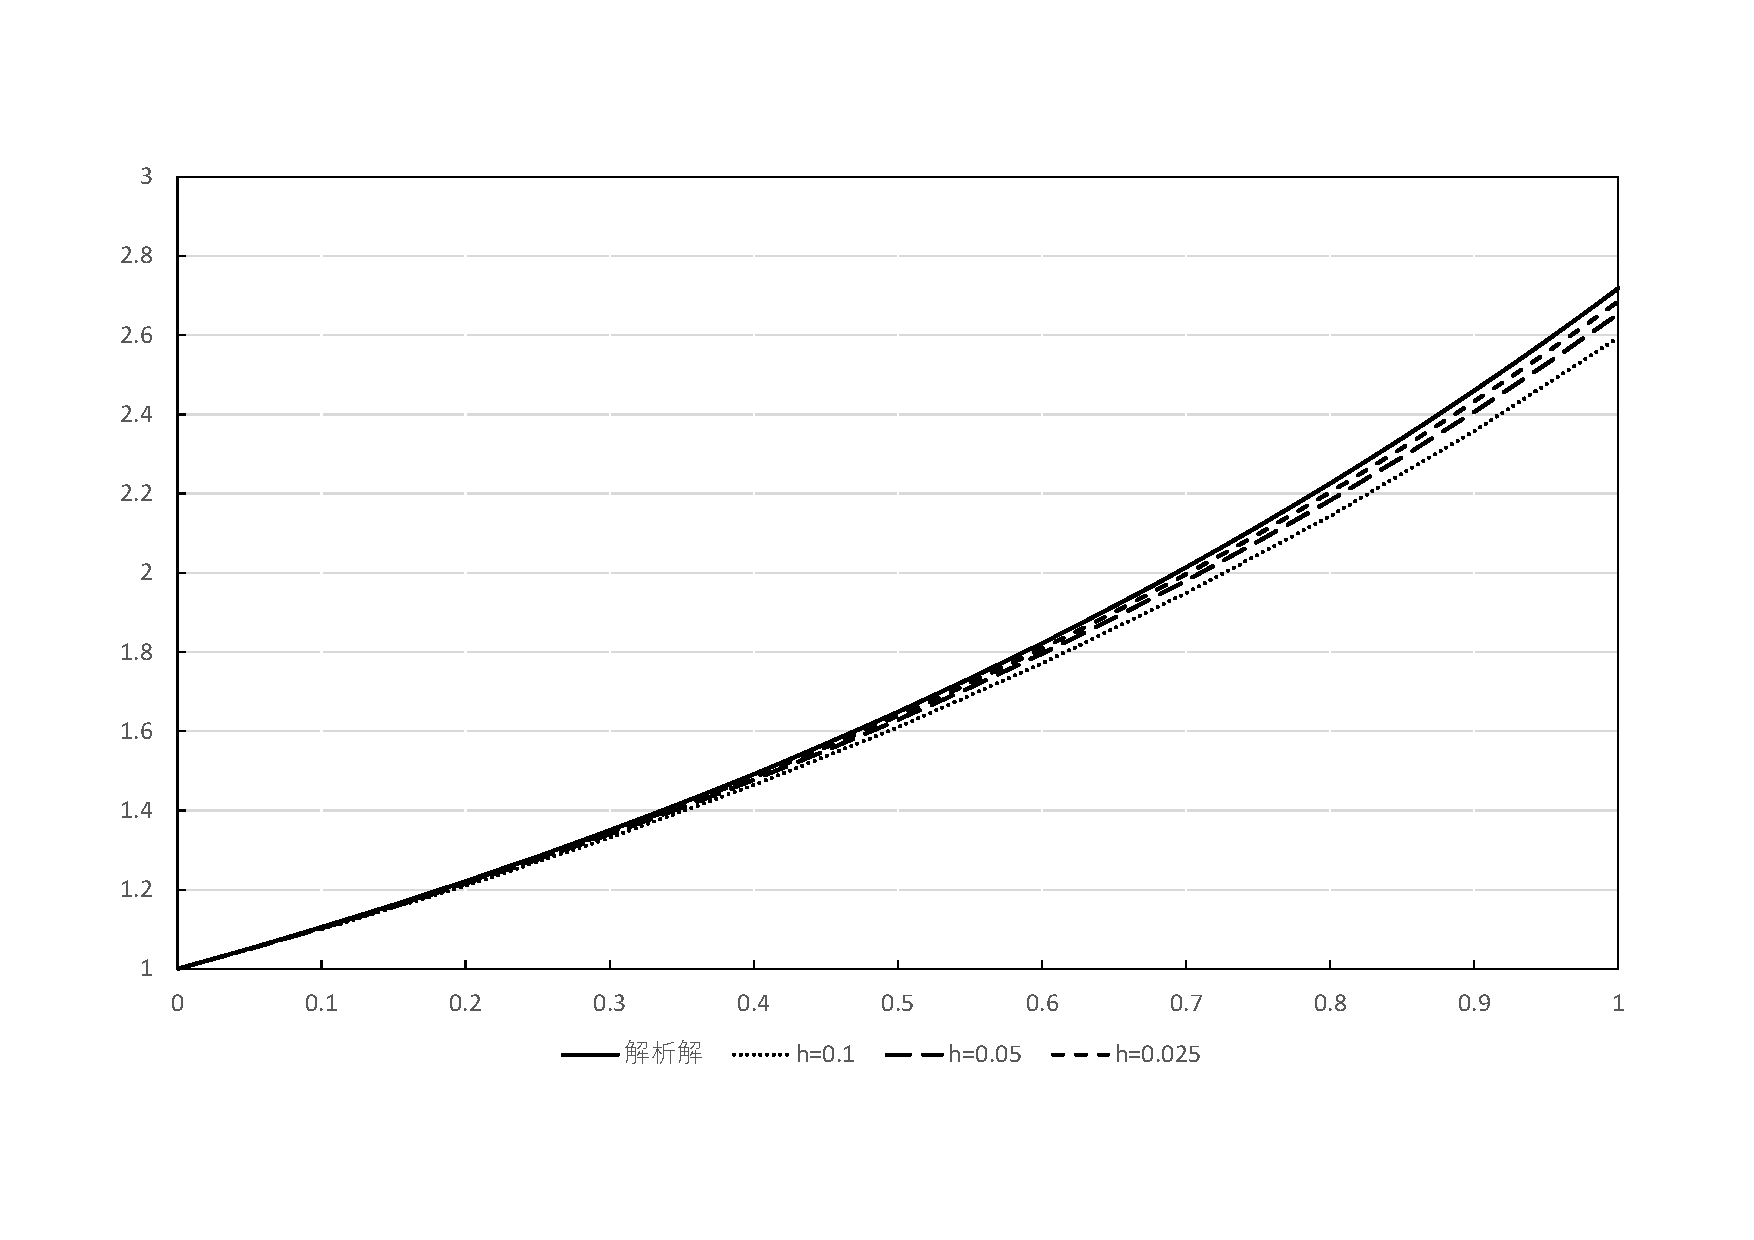
\includegraphics[width=12cm]{img/kadai3.png}
\caption{オイラー法  解析解との差}
\label{fig:kadai3}
\end{figure}

刻み幅を小さくするほど実線で表された解析解に近づく事がわかる。しかし、$t$の値が大きくなるにつれて差が大きくなってしまう。

図\ref{fig:kadai4}はオイラー法で式(\ref{eq:kadai345})を解いて、刻み幅を$h=0.1,h=0.05,h=0.025$に変更していき同じ$t$の値をグラフにプロットしたものである。

\begin{figure}[H]
\centering
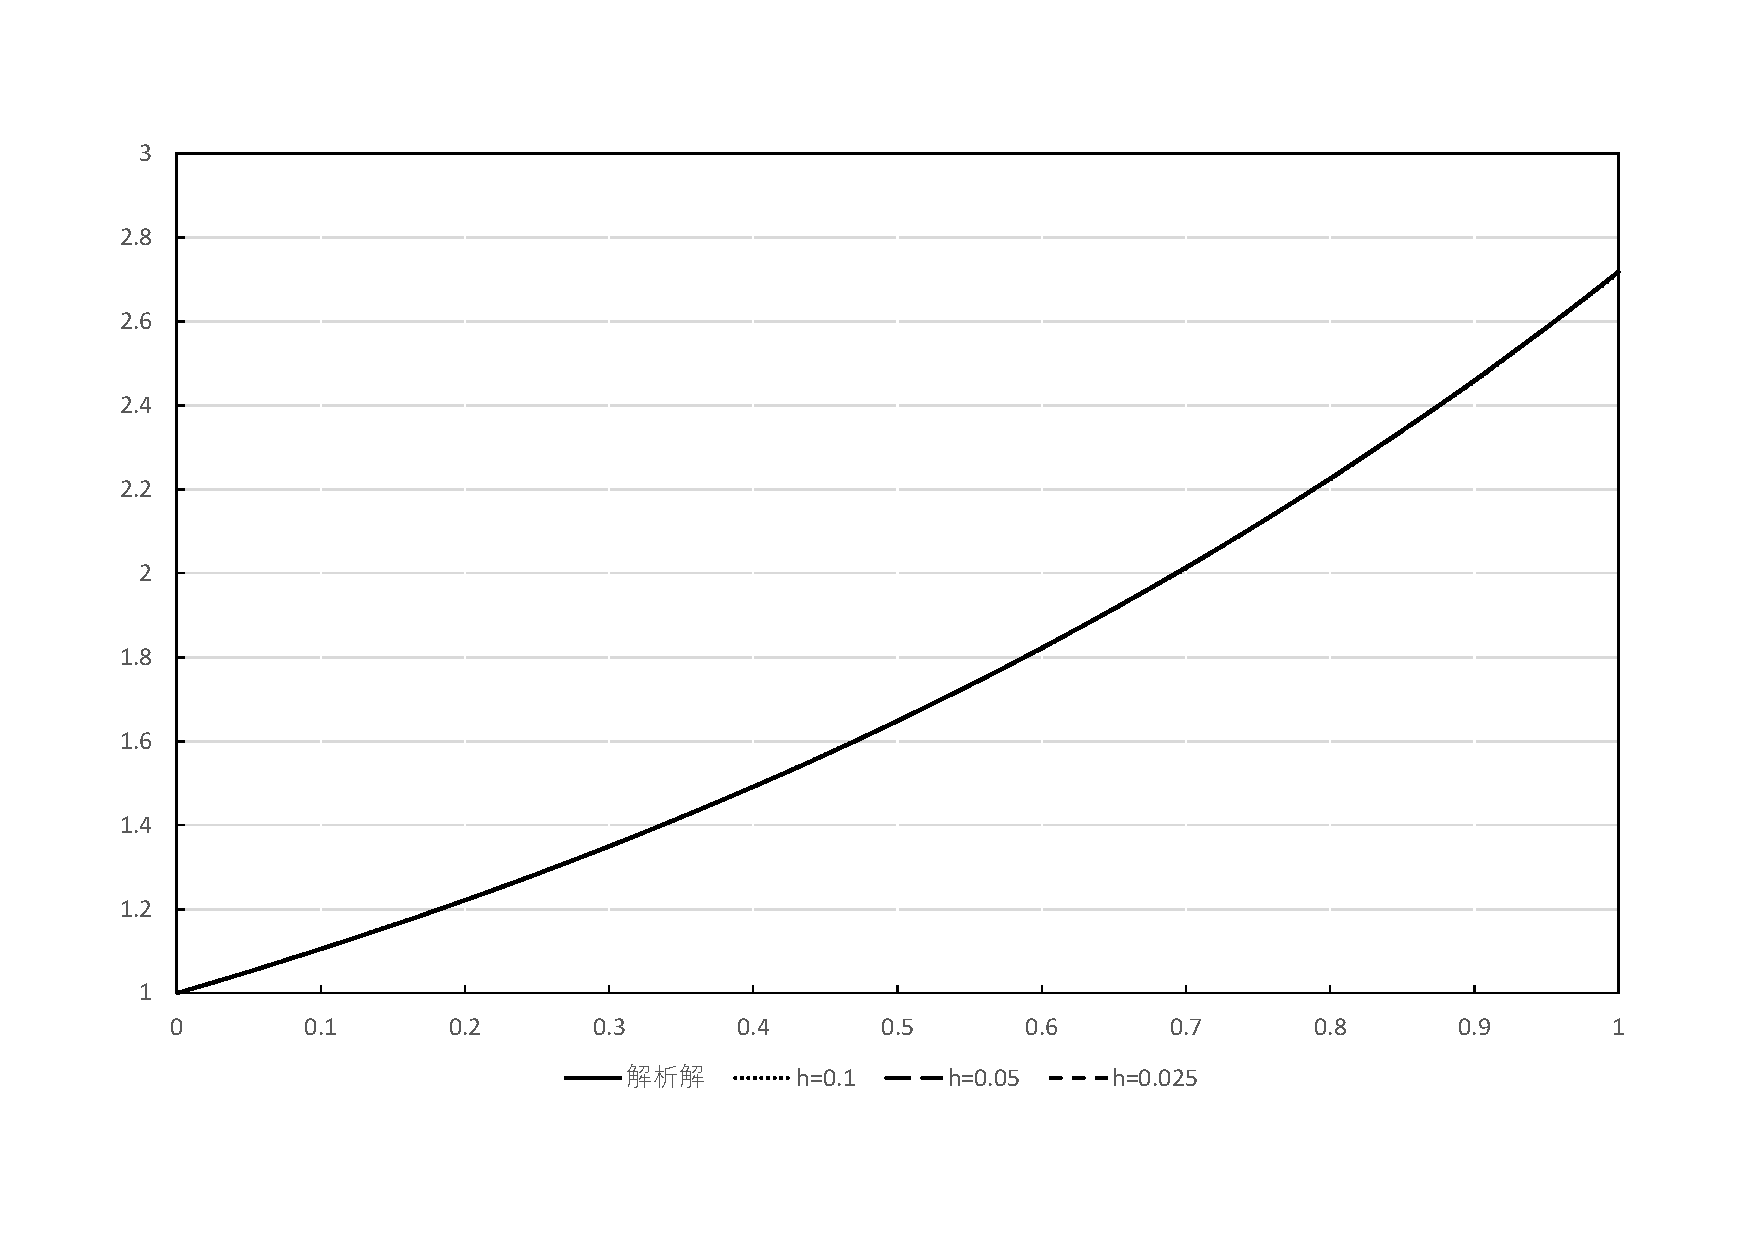
\includegraphics[width=12cm]{img/kadai4.png}
\caption{ホイン法  解析解との差}
\label{fig:kadai4}
\end{figure}

数値解は解析解とほぼ一致していることがわかる。


図\ref{fig:kadai5}はオイラー法で式(\ref{eq:kadai345})を解いて、刻み幅を$h=0.1,h=0.05,h=0.025$に変更していき同じ$t$の値をグラフにプロットしたものである。

\begin{figure}[H]
\centering
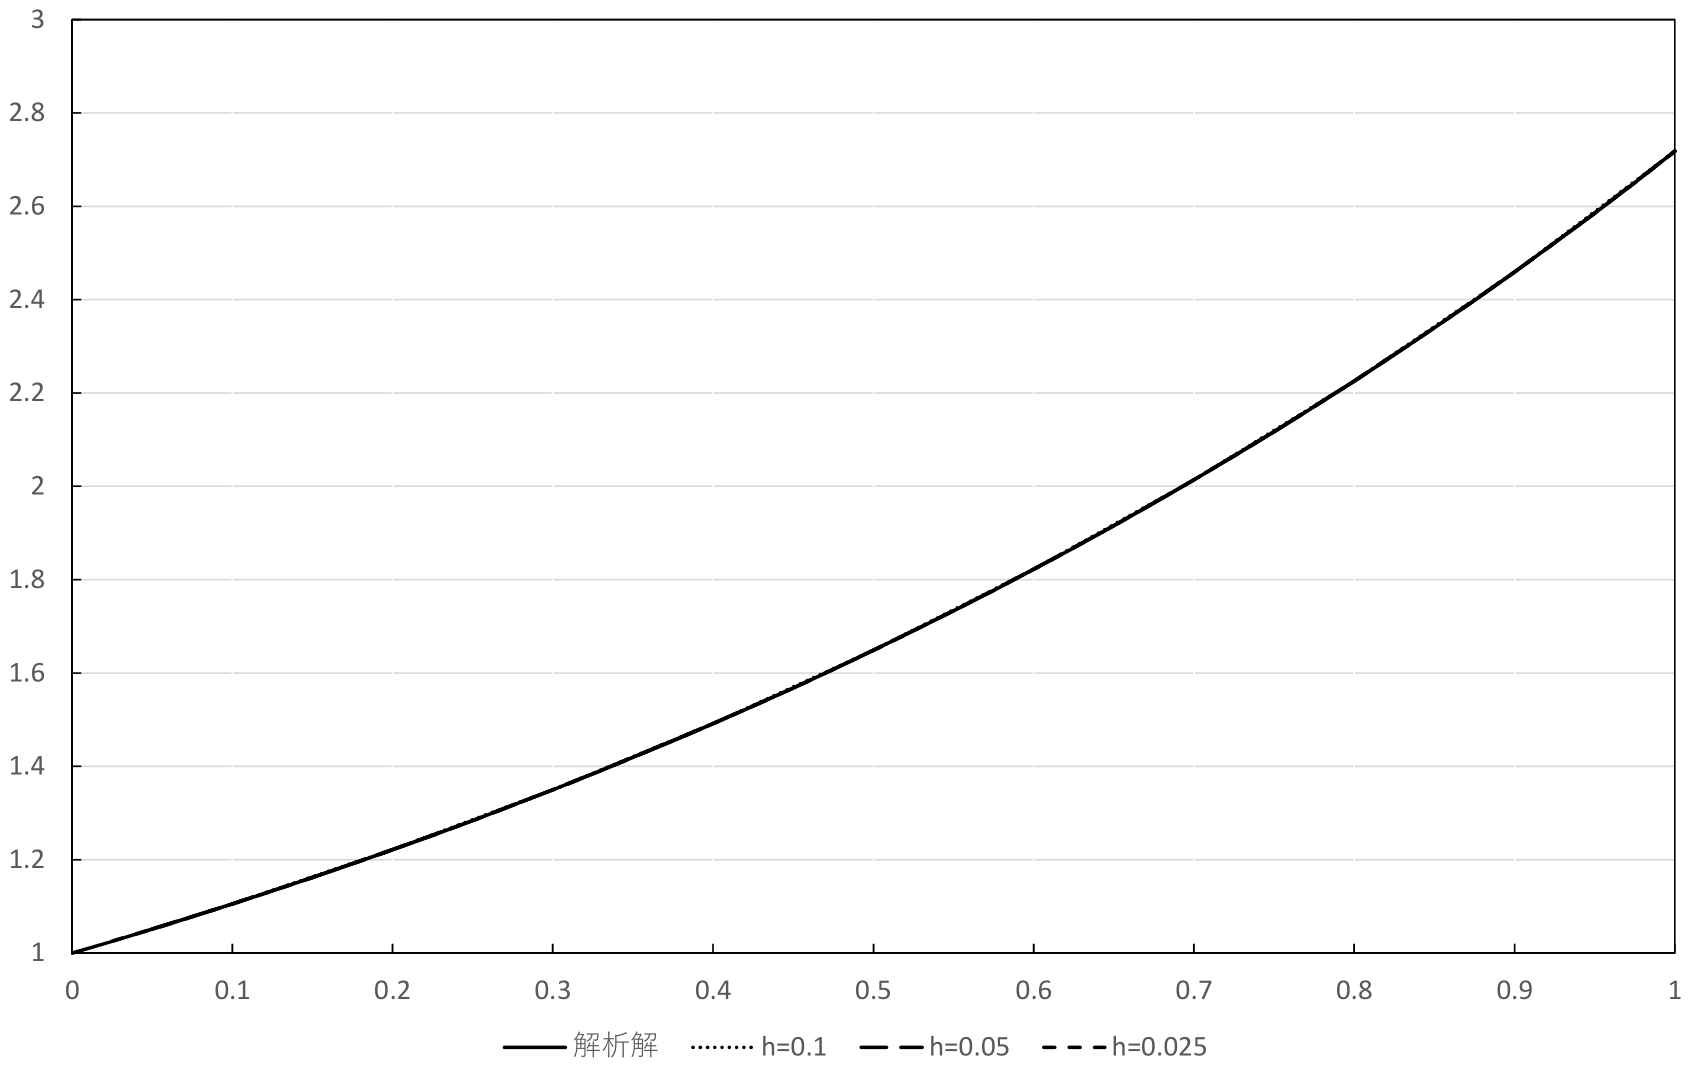
\includegraphics[width=12cm]{img/kadai5.png}
\caption{ルンゲ・クッタ法  解析解との差}
\label{fig:kadai5}
\end{figure}

数値解は解析解とほぼ一致していることがわかる。

\appendix
\section{課題3、4、5実行結果}
\label{kadai345}
課題3、4、5実行結果を以下に示す。

\begin{oframed}
\verbatimtabinput[2]{result/kadai345full.txt}
\end{oframed}



\end{document}